\setcounter{section}{6}

\Needspace{5\baselineskip}
\hypertarget{grpo}{%
\section{GRPO}\label{grpo}}

GRPO is a PPO variant without a critic network. It exploits LLMs' strong parallel-generation capability to estimate values without bias through Monte Carlo methods, replacing potentially biased neural estimates. Removing one network substantially reduces GPU memory while preserving mathematical training stability.

\Needspace{5\baselineskip}
\hypertarget{i.-monte-carlo-value-estimation}{%
\subsection{I. Monte Carlo Value Estimation}\label{i.-monte-carlo-value-estimation}}

\Needspace{5\baselineskip}
In reinforcement learning, the advantage function \(A(s,a)\) is defined as:

\[
A(s,a)=Q(s,a)-V(s)
\]

\Needspace{5\baselineskip}
GRPO calculates it as follows:

\begin{itemize}
\tightlist
\item
  Estimating \(Q(s,a)\): for the \(i\)-th sampled output \(o_i\), its actual reward \(r_i\) is one Monte Carlo sample of action value \(Q(s,a)\), an unbiased estimate.
\item
  Estimating \(V(s)\): calculate the group's mean reward \(\bar{r}=\frac{1}{G}\sum_{j=1}^{G}r_j\).
\end{itemize}

\Needspace{5\baselineskip}
By the law of large numbers, as \(G\to\infty\):

\[
\bar{r}\to \mathbb{E}[R\mid s]=V(s)
\]

\Needspace{5\baselineskip}
Thus, \(A_i=r_i-\bar{r}\) essentially means:

\[
\text{Advantage}\approx \text{Sampled }Q(s,a)-\text{Monte Carlo Estimated }V(s)
\]

Monte Carlo's advantage is unbiasedness. In Q-network updates, bias in one state--action value affects other Q-value updates and easily accumulates; Monte Carlo does not have this problem.

If direct, unbiased Monte Carlo estimation is so good, why does PPO train a critic to predict \(V(s)\)?

The central reason is variance.

Traditional RL faces single-sample estimation. In robot control or Atari games, usually only one trajectory can be sampled from current \(s\).

\begin{itemize}
\tightlist
\item
  If one sample yields \(r\), using \(r\) directly as \(Q\) has enormous variance.
\item
  Without a critic, historical average rewards must provide the baseline.
\item
  This makes training unstable and convergence slow.
\end{itemize}

\Needspace{5\baselineskip}
PPO uses actor--critic learning with \(V_{\phi}(s)\):

\begin{itemize}
\tightlist
\item
  Advantage: reduced variance. The critic has seen many similar states and predicts smoothly and stably.
\item
  Disadvantage: bias. A poorly fitted critic gives an incorrect baseline, misdirecting actor updates, while doubling memory use.
\end{itemize}

GRPO can return to Monte Carlo because of a distinctive engineering property of LLM inference: one prompt can cheaply produce varied outcomes.

In robotics, repeating an action 64 times under exactly identical conditions is difficult because the environment is irreversible. For LLMs, one can simply set \texttt{num\_return\_sequences=64}.

\Needspace{5\baselineskip}
Although Monte Carlo usually has high variance, GRPO controls it without a critic:

\begin{enumerate}
\def\labelenumi{\arabic{enumi}.}
\tightlist
\item
  Group sampling with sufficiently large \(G\): estimate \(V(s)\) from \(G\) samples rather than one; DeepSeek, for example, uses \(G=64\). By the central limit theorem, the sample mean's variance is \(\frac{1}{G}\) of a single sample's variance. Increasing \(G\) directly reduces Monte Carlo variance.
\item
  Group normalization: \(\frac{r_i-\bar{r}}{\sigma_R}\) subtracts the mean and divides by the standard deviation. This dynamically scales rewards, further stabilizing gradient magnitudes in a way similar to batch normalization.
\end{enumerate}

\Needspace{5\baselineskip}
\hypertarget{ii.-architecture-and-formulation}{%
\subsection{II. Architecture and Formulation}\label{ii.-architecture-and-formulation}}

\Needspace{5\baselineskip}
For rigorous derivation, use the following notation:

\begin{itemize}
\tightlist
\item
  \(q\): the input question (prompt), sampled from \(P(Q)\).
\item
  \(G\): group size, the number of outputs sampled per question.
\item
  \(o_i\): output sequence \(i\) for the same \(q\), where \(i\in\{1,\ldots,G\}\).
\item
  \(T_i\): the length of the \(i\)-th output sequence \(o_i\) in tokens.
\item
  \(o_{i,t}\): token \(t\) of \(o_i\).
\item
  \(\pi_{\theta}\): the current policy model being optimized.
\item
  \(\pi_{\theta_{\mathrm{old}}}\): the old policy used for sampling.
\item
  \(\pi_{\mathrm{ref}}\): the reference model, usually SFT, for the KL constraint.
\item
  \(r_i\): the full reward for output sequence \(i\), from a reward model or environment.
\item
  \(A_i\): the advantage of output sequence \(i\).
\end{itemize}

\begin{figure}[htbp]
\centering
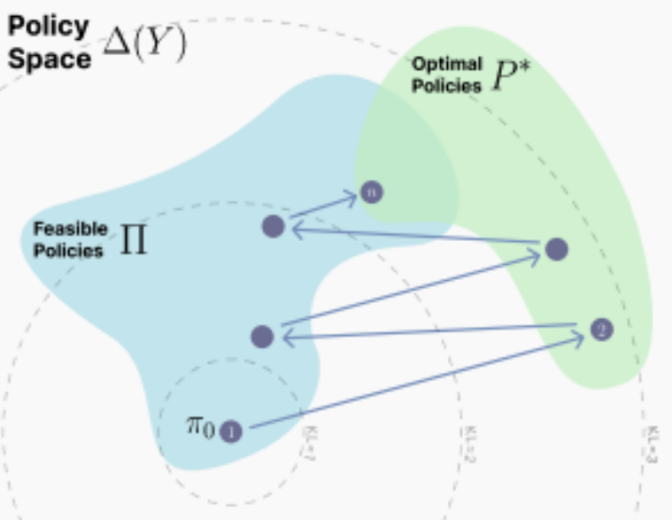
\includegraphics{images/image-0022.png}
\caption{Comparison of PPO and GRPO architectures}
\end{figure}

The diagram shows that PPO trains an additional value model to estimate the baseline. GRPO freezes the reference model and estimates the baseline from within-group rewards, eliminating the critic.

\Needspace{5\baselineskip}
\hypertarget{group-sampling-in-place-of-expectation-calculation}{%
\subsubsection{1. Group Sampling in Place of Expectation Calculation}\label{group-sampling-in-place-of-expectation-calculation}}

\Needspace{5\baselineskip}
For input \(q\), sample \(G\) outputs using \(\pi_{\theta_{\mathrm{old}}}\):

\[
\{o_1,o_2,\ldots,o_G\}\sim \pi_{\theta_{\mathrm{old}}}(O\mid q)
\]

Then calculate rewards \(\{r_1,r_2,\ldots,r_G\}\).

\Needspace{5\baselineskip}
\hypertarget{advantage-estimation}{%
\subsubsection{2. Advantage Estimation}\label{advantage-estimation}}

This replaces the critic. Traditional A2C/PPO predicts the baseline with \(V_{\phi}(s)\), while GRPO uses the current group's mean reward.

\Needspace{5\baselineskip}
Calculate the advantage \(A_i\) of sample \(i\):

\[
A_i=\frac{r_i-\mu_{\mathrm{group}}}{\sigma_{\mathrm{group}}+\epsilon}
\]

Here, \(\mu_{\mathrm{group}}\) and \(\sigma_{\mathrm{group}}\) are the current group's reward mean and standard deviation.

Standard-deviation normalization accounts for potentially incomparable scoring schemes across question types. It can also cause problems: for very difficult or easy questions whose responses score almost identically, the question's weight may be artificially amplified. Subsequent engineering improvements address this.

\Needspace{5\baselineskip}
\hypertarget{objective-and-length-normalization}{%
\subsubsection{3. Objective and Length Normalization}\label{objective-and-length-normalization}}

\Needspace{5\baselineskip}
The objective \(J(\theta)\) is:

\[
\begin{aligned}
\mathcal{J}_{\mathrm{GRPO}}(\theta)
&=\mathbb{E}_{q\sim P(Q),\{o_i\}_{i=1}^{G}\sim\pi_{\theta_{\mathrm{old}}}(O\mid q)} \\
&\quad \left[
\frac{1}{G}\sum_{i=1}^{G}\frac{1}{T_i}\sum_{t=1}^{T_i}
\right. \\
&\qquad \left.
\left(
\min\!\bigl(\rho_{i,t}A_i,\mathrm{clip}(\rho_{i,t},1-\epsilon,1+\epsilon)A_i\bigr)
-\beta D_{\mathrm{KL},t}
\right)
\right]
\end{aligned}
\]

Clipping and KL coexist but differ in purpose. Clipping limits a single gradient update to avoid excessive per-iteration policy change and training collapse. KL constrains cumulative drift from the initial reference, preventing language degradation in pursuit of higher reward.

\(\rho_{i,t}\) is the current-to-old policy probability ratio, and \(D_{\mathrm{KL},t}\) the KL penalty at the current token. Taking the expectation over old-policy samples gives the KL constraint between policy and reference. Vocabulary-wide enumeration is unnecessary: it usually serves to compute an expectation, already approximated by group-based Monte Carlo sampling.

Reverse rather than forward KL is used because \(KL(\pi_{\theta}\Vert\pi_{\mathrm{ref}})\) strongly penalizes regions assigned high probability by the current policy but low probability by the reference. This produces mode-seeking behavior, concentrating the new distribution on specific modes within the pretrained high-probability region. Leaving that region often yields gibberish or semantically abnormal content, that is, mode collapse. Forward KL instead covers the pretrained high-probability region, showing mean-seeking behavior. RL's acquired space is often a subset of pretraining's space, possibly one reason RL struggles to produce skills completely absent from pretraining.

Inside the brackets, outputs 1 through \(G\) for the same input are averaged, followed by length normalization, another key feature of GRPO.

\Needspace{5\baselineskip}
Standard policy gradients optimize expected total reward:

\[
J=\mathbb{E}_{\tau\sim\pi_{\theta}}[R(\tau)]
\]

\Needspace{5\baselineskip}
Ignoring the baseline, the gradient is:

\[
\nabla J\approx \sum_{t=1}^{T}\nabla\log\pi_{\theta}(a_t\mid s_t)\cdot R
\]

The gradient of objective \(J\) sums contributions calculated from the policy for every action. If the gradient of \(J\) for each action has magnitude 1, a sequence of length 100 gives roughly ten times the gradient of a sequence of length 10, letting long sequences dominate updates. For one question, however, each answer sequence should contribute equally, so divide by length \(T\):

\[
\nabla J_{\mathrm{GRPO}}\approx \frac{1}{T}\sum_{t=1}^{T}\nabla\log\pi_{\theta}(a_t\mid s_t)\cdot A
\]

\Needspace{5\baselineskip}
This creates another problem: dividing \(J\)'s gradient by \(T\) means dividing \(J\) itself by \(T\), changing the objective to ``expected reward per token.'' This encourages many useless tokens in incorrect answers, because:

Positive advantage means a correct result and a positive objective. Since expected per-token reward has denominator \(T\), maximizing it favors short correct answers, which generate larger gradient updates.

Negative advantage means an incorrect result and a negative objective. To increase the objective (reduce the magnitude of the penalty), optimization favors longer answers because the objective divides by a larger \(T\). Such answers receive weaker negative penalties and gradient pressure.

\Needspace{5\baselineskip}
\hypertarget{iii.-bias-in-advantage-estimation-and-remedies}{%
\subsection{III. Bias in Advantage Estimation and Remedies}\label{iii.-bias-in-advantage-estimation-and-remedies}}

GRPO's advantage estimate appears unbiased but often underestimates difficult questions and overestimates easy ones. Suppose eight paths are sampled for a hard problem with 1\% success probability, reward 1 for success and 0 for failure. Eight failures produce no gradient. With one success, its advantage is \(1-\frac{1}{8}=\frac{7}{8}\), whereas the true advantage is \(1-\frac{1}{100}=\frac{99}{100}\). Easy questions reverse this: at 99\% success probability with one failure, successful samples have advantage \(\frac{1}{8}\) rather than the true \(\frac{1}{100}\).

Larger coefficients for difficult-question advantages and smaller ones for easy questions can make estimation as unbiased as possible.

\FloatBarrier
\Needspace{5\baselineskip}
\hypertarget{references-85}{%
\subsection{References}\label{references-85}}

\vspace{0.25em}
\begin{itemize}
\tightlist
\item
  Shao, Z., Wang, P., Zhu, Q., et al.~(2024). \href{https://arxiv.org/abs/2402.03300}{DeepSeekMath: Pushing the Limits of Mathematical Reasoning in Open Language Models}. arXiv:2402.03300.
\end{itemize}

\clearpage
